\documentclass[tikz]{standalone}
\usepackage{amssymb}
\begin{document}

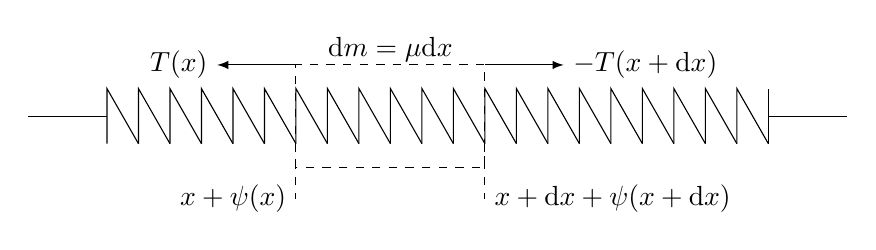
\begin{tikzpicture}[>=latex]
	\def\pas{.4}
	\def\nspire{20}
	\def\springh{.7}

	% ressort
	\foreach \i in {0,...,\nspire} {
		\draw (\i*\pas,0) -- (\i*\pas,\springh) -- (\i*\pas+\pas,0);
	}
	\draw (\pas*\nspire+\pas,0) -- (\pas*\nspire+\pas,\springh);
	\draw (-1,\springh/2) -- (0,\springh/2);
	\draw (\pas*\nspire+\pas,\springh/2) -- (\pas*\nspire+\pas+1,\springh/2);

	% dx
	\def\start{6}
	\def\stop{12}
	\draw[dashed] (\start*\pas,-.3) rectangle (\stop*\pas,\springh+.3);

	% abscisses
	\draw[dashed] (\start*\pas,0) -- (\start*\pas,-.7) node[below,left] {$x+\psi(x)$};
	\draw[dashed] (\stop*\pas,0) -- (\stop*\pas,-.7) node[below,right] {$x+\mathrm{d}x+\psi(x+\mathrm{d}x)$};

	% dm
	\draw (\start*0.5*\pas+\stop*.5*\pas,\springh+.5) node {$\mathrm{d}m = \mu\mathrm{d}x$};

	% forces
	\draw[->] (\start*\pas,\springh+.3) -- ++(-1,0) node[left] {$T(x)$};
	\draw[->] (\stop*\pas,\springh+.3) -- ++(1,0) node[right] {$-T(x+\mathrm{d}x)$};

\end{tikzpicture}

\end{document}
